\autsection{General Approach}{Nelián Colón}

At first, the team will be developing different parts of
the system as they are all loosely coupled. Test driven development will be
done, meaning that after each part gets successfully developed and unit tested,
only then they are integrated and tested from a bigger perspective. The project
is divided into 4 major parts, these are: front end client, back end server,
test framework, and repository manager, as shown in Figure~\ref{arqu}. The team
will be using a single cloud hosted Git repository (GitHub) where the project's
code will live. Moreover, the
team will follow the Scrum agile development process.

\begin{figure}[H]
	\centering
	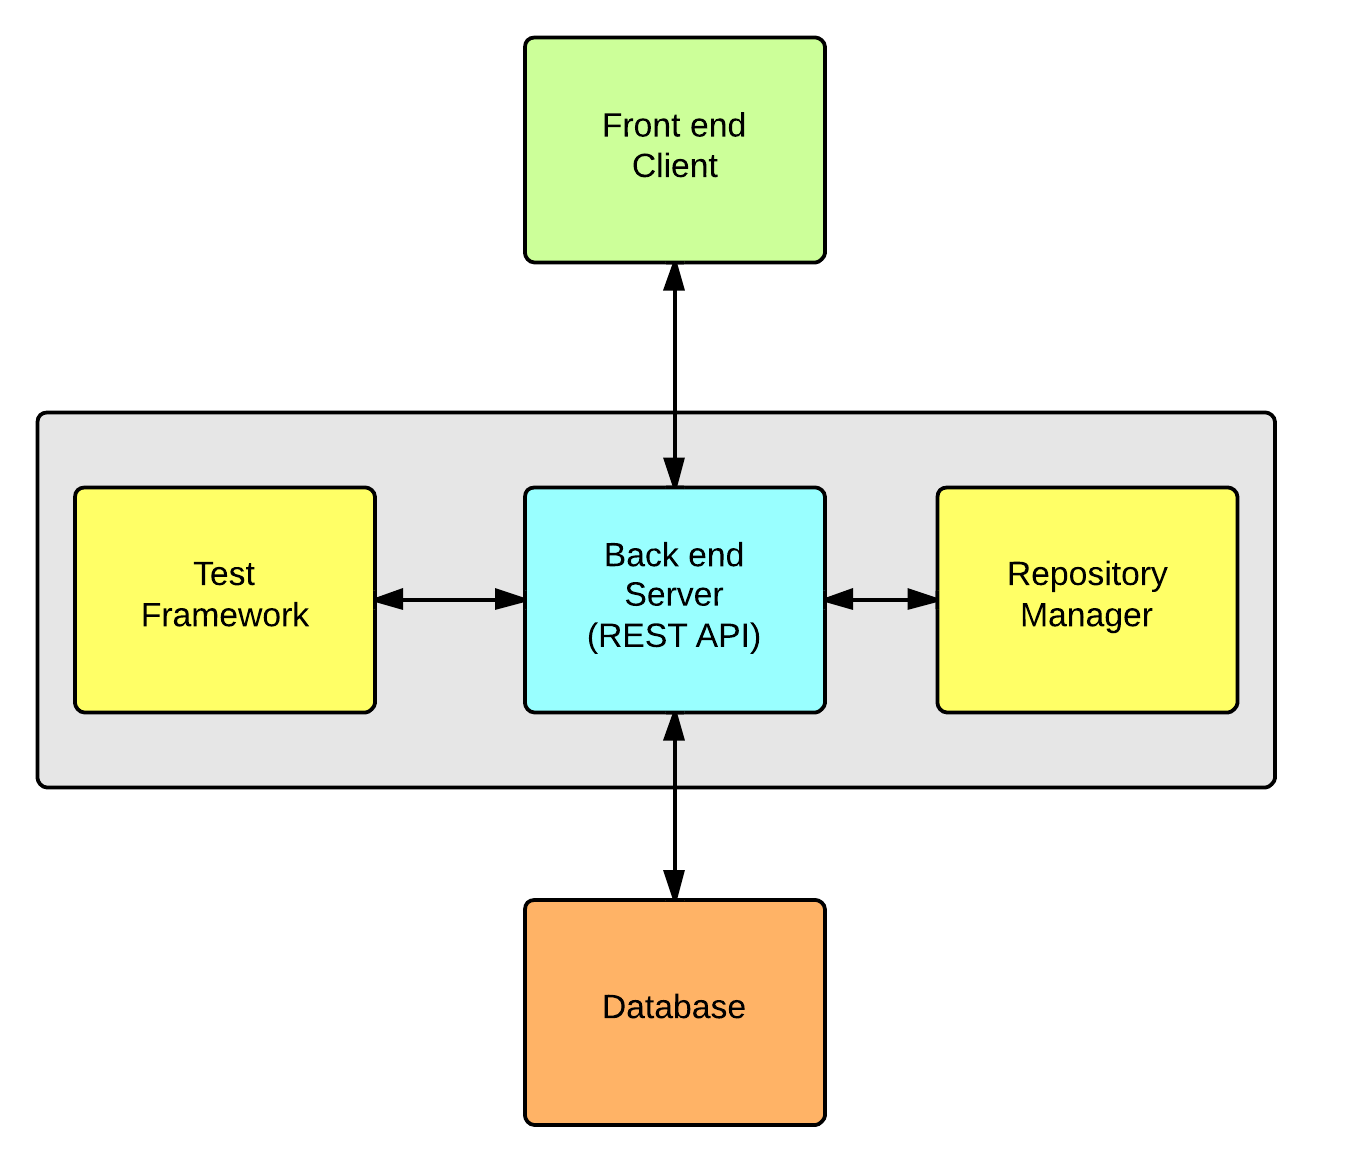
\includegraphics[scale=0.15]{img/bigArquitectOverview}
	\caption{General overview of the system\label{arqu}}
\end{figure}

\subsection{Team Management}

As formerly mentioned, the team will follow the Scrum agile development process.
Meetings will be held at the start and end of each sprint, these meeting are
sprint planning and sprint retrospective. Each task will have a leader and an
assistant. The leader of each task is completely responsible for the task and
the assistant will assist whenever the leader gets stuck on a problem. Tasks
will have a weight that is going to be decided during the sprint planning
meeting. Table~\ref{tasks} contains the main tasks distribution for the project.
For a more detailed list of task distribution see the Gantt Chart included as a
separate file.

\begin{center}
\setlength{\extrarowheight}{1.5pt}
  \begin{longtable}{|m{3.25in}|c|c|c|}
 \caption{Task Distribution \label{tasks}} \\
   \hline
  
  \centering Task Title & Nelián & Samuel & Daniel \\
  \hline \hline \endfirsthead
  
     \hline

	\centering Task Title & Nelián & Samuel & Daniel \\  
	\hline \hline \endhead
  
  \endfoot  
  
  Project Management and Team Organization & Lead & Assist & \\ \hline
  Web Front end & & Lead & Assist \\ \hline
  Back end Server & & Assist & Lead \\ \hline
  Test Framework & Assist & & Lead \\ \hline
  Accounts \& Repositories & Lead & Assist & \\ \hline
   \end{longtable}
\end{center}

\subsection{Testing and Quality Control Procedures}

To ensure the quality of the software product, the team will employ both static
and dynamic testing. Static testing will be performed via code reviews for every
single Git repository commit. The reviewers will be the other two team members
that do not submit the comment, hence, every team member will review each change
for commit. The review will include running the change in each of the team
member's work station, and visually inspecting the code. This will help detect
bugs and also maintain good coding guidelines and style. Dynamic testing will be
performed via different testing levels. The first level will be Unit testing,
which will be required for every commit in which unit tests are applicable. If a
unit test is not included in an applicable change, then the commit will be
unapproved by the other team members, and will not be pushed to the main
repository. The next level of testing will be integration testing, which will
occur even before integration begins. The last testing level will be system
testing, which will occur on Amazon's infracture on every push of the
repository. Nightly builds will be uploaded to Amazon's infrastructure to ensure
that the system is working every time, and system tests will run after the
change is built remotely.

\subsection{Documentation Standards}
To document the design of the system, the team will use the Unified Modeling Language (UML) standard.